\documentclass[12pt]{article}
\usepackage[utf8]{inputenc}
\usepackage[utf8]{inputenc}
\usepackage{amsmath}
\usepackage{amsthm}
\usepackage{amssymb}
\usepackage{geometry}
\usepackage{amsfonts}
\usepackage{mathrsfs}
\usepackage{bm}
\usepackage{hyperref}
\usepackage{float}
\usepackage[dvipsnames]{xcolor}
\usepackage[inline]{enumitem}
\usepackage{mathtools}
\usepackage{changepage}
\usepackage{graphicx}
\usepackage{caption}
\usepackage{subcaption}
\usepackage{lipsum}
\usepackage{tikz}
\usetikzlibrary{matrix, patterns, decorations.pathreplacing, calligraphy}
\usepackage{tikz-cd}
\usepackage[nameinlink]{cleveref}
\geometry{
headheight=15pt,
left=60pt,
right=60pt
}
\setlength{\emergencystretch}{20pt}
\usepackage{fancyhdr}
\pagestyle{fancy}
\fancyhf{}
\lhead{}
\chead{Section 6.2 Exercises}
\rhead{\thepage}
\hypersetup{
    colorlinks=true,
    linkcolor=blue,
    urlcolor=blue
}

\theoremstyle{definition}
\newtheorem*{remark}{Remark}

\newtheoremstyle{exercise}
    {}
    {}
    {}
    {}
    {\bfseries}
    {.}
    { }
    {\thmname{#1}\thmnumber{#2}\thmnote{ (#3)}}
\theoremstyle{exercise}
\newtheorem{exercise}{Exercise 6.2.}

\newtheoremstyle{solution}
    {}
    {}
    {}
    {}
    {\itshape\color{magenta}}
    {.}
    { }
    {\thmname{#1}\thmnote{ #3}}
\theoremstyle{solution}
\newtheorem*{solution}{Solution}

\Crefformat{exercise}{#2Exercise 6.2.#1#3}

\newcommand{\interior}[1]{%
  {\kern0pt#1}^{\mathrm{o}}%
}
\newcommand{\ts}{\textsuperscript}
\newcommand{\setcomp}[1]{#1^{\mathsf{c}}}
\newcommand{\quand}{\quad \text{and} \quad}
\newcommand{\N}{\mathbf{N}}
\newcommand{\Z}{\mathbf{Z}}
\newcommand{\Q}{\mathbf{Q}}
\newcommand{\I}{\mathbf{I}}
\newcommand{\R}{\mathbf{R}}
\newcommand{\C}{\mathbf{C}}

\DeclarePairedDelimiter\abs{\lvert}{\rvert}
% Swap the definition of \abs* and \norm*, so that \abs
% and \norm resizes the size of the brackets, and the 
% starred version does not.
\makeatletter
\let\oldabs\abs
\def\abs{\@ifstar{\oldabs}{\oldabs*}}
%
\let\oldnorm\norm
\def\norm{\@ifstar{\oldnorm}{\oldnorm*}}
\makeatother

\DeclarePairedDelimiter\paren{(}{)}
\makeatletter
\let\oldparen\paren
\def\paren{\@ifstar{\oldparen}{\oldparen*}}
\makeatother

\DeclarePairedDelimiter\bkt{[}{]}
\makeatletter
\let\oldbkt\bkt
\def\bkt{\@ifstar{\oldbkt}{\oldbkt*}}
\makeatother

\DeclarePairedDelimiter\set{\{}{\}}
\makeatletter
\let\oldset\set
\def\set{\@ifstar{\oldset}{\oldset*}}
\makeatother

\setlist[enumerate,1]{label={(\alph*)}}

\begin{document}

\section{Section 6.2 Exercises}

Exercises with solutions from Section 6.2 of \hyperlink{ua}{[UA]}.

\begin{exercise}
\label{ex:1}
    Let
    \[
        f_n(x) = \frac{nx}{1 + nx^2}.
    \]
    \begin{enumerate}
        \item Find the pointwise limit of \( (f_n) \) for all \( x \in (0, \infty) \).

        \item Is the convergence uniform on \( (0, \infty) \)?

        \item Is the convergence uniform on \( (0, 1) \)?

        \item Is the convergence uniform on \( (1, \infty) \)?
    \end{enumerate}
\end{exercise}

\begin{solution}
    \begin{enumerate}
        \item Fix \( x \in (0, \infty) \). Then
        \[
            \lim_{n \to \infty} f_n(x) = \lim_{n \to \infty} \frac{nx}{1 + nx^2} = \lim_{n \to \infty} \frac{x}{\tfrac{1}{n} + x^2} = \frac{1}{x}.
        \]
        Thus, letting \( f : (0, \infty) \to \R \) be the function given by \( f(x) = \tfrac{1}{x} \), we see that \( (f_n) \) converges pointwise to \( f \).

        \item The convergence is not uniform on \( (0, \infty) \). To argue this, it is worthwhile to negate the definition of uniform convergence. A sequence of functions \( (f_n : A \to \R) \) does not converge uniformly to a function \( f : A \to \R \) if there exists an \( \epsilon > 0 \) such that for all \( N \in \N \), we can find an \( x \in A \) and an \( n \geq N \) such that \( \abs{f_n(x) - f(x)} \geq \epsilon \). In symbols:
        \[
            (\exists \epsilon > 0)(\forall N \in \N)(\exists x \in A)(\exists n \geq N)(\abs{f_n(x) - f(x)} \geq \epsilon).
        \]
        Returning to the exercise, let \( N \in \N \) be given and observe that
        \[
            \abs{f_N \paren{ \tfrac{1}{N} } - f \paren{ \tfrac{1}{N} }} = \frac{1}{\tfrac{1}{N} \paren{ 1 + \tfrac{1}{N} }} \geq \frac{1}{2}.
        \]

        \item The convergence is not uniform on \( (0, 1) \) and the proof of this is almost identical to part (b); this time, given \( N \in \N \), take \( n = N + 1 \) and \( x = \tfrac{1}{N + 1} \) to ensure \( x \in (0, 1) \).

        \item The convergence is uniform on \( (1, \infty) \). Let \( \epsilon > 0 \) be given and let \( N \in \N \) be such that \( N > \tfrac{1}{\epsilon} - 1 \). Then for all \( x \in (1, \infty) \) and all \( n \geq N \), we have
        \[
            \abs{f_n(x) - f(x)} = \frac{1}{x(1 + nx^2)} \leq \frac{1}{1 + n} \leq \frac{1}{1 + N} < \epsilon.
        \]
    \end{enumerate}
\end{solution}

\begin{exercise}
\label{ex:2}
    \begin{enumerate}
        \item Define a sequence of functions on \( \R \) by
        \[
            f_n(x) = \begin{cases}
                1 & \text{if } x = 1, \tfrac{1}{2}, \tfrac{1}{3}, \ldots, \tfrac{1}{n} \\
                0 & \text{otherwise}
            \end{cases}
        \]
        and let \( f \) be the pointwise limit of \( f_n \).

        Is each \( f_n \) continuous at zero? Does \( f_n \to f \) uniformly on \( \R \)? Is \( f \) continuous at zero?

        \item Repeat this exercise using the sequence of functions
        \[
            g_n(x) = \begin{cases}
                x & \text{if } x = 1, \tfrac{1}{2}, \tfrac{1}{3}, \ldots, \tfrac{1}{n} \\
                0 & \text{otherwise}.
            \end{cases}
        \]

        \item Repeat the exercise once more with the sequence
        \[
            h_n(x) = \begin{cases}
                1 & \text{if } x = \tfrac{1}{n} \\
                x & \text{if } x = 1, \tfrac{1}{2}, \tfrac{1}{3}, \ldots, \tfrac{1}{n - 1} \\
                0 & \text{otherwise}.
            \end{cases}
        \]
        In each case, explain how the results are consistent with the content of the Continuous Limit Theorem (Theorem 6.2.6).
    \end{enumerate}
\end{exercise}

\begin{solution}
    \begin{enumerate}
        \item Define \( f : \R \to \R \) by
        \[
            f(x) = \begin{cases}
                1 & \text{if } x = 1, \tfrac{1}{2}, \tfrac{1}{3}, \ldots, \\
                0 & \text{otherwise}.
            \end{cases}
        \]
        Then \( (f_n) \) converges to \( f \) pointwise: if \( x \not\in \set{ 1, \tfrac{1}{2}, \tfrac{1}{3}, \ldots } \), then
        \[
            \abs{f_n(x) - f(x)} = \abs{0 - 0} = 0,
        \]
        and if \( x = \tfrac{1}{N} \) for some \( N \in \N \), then for all \( n \geq N \) we have
        \[
            \abs{f_n(x) - f(x)} = \abs{1 - 1} = 0.
        \]
        Each \( f_n \) is continuous at zero, since each \( f_n \) is identically zero on the interval \( \paren{ -\infty, \tfrac{1}{n} } \), however \( f \) is evidently not continuous at zero. It follows that the convergence \( f_n \to f \) cannot be uniform, otherwise the Continuous Limit Theorem (Theorem 6.2.6) would be contradicted.

        \item Define \( g : \R \to \R \) by
        \[
            g(x) = \begin{cases}
                x & \text{if } x = 1, \tfrac{1}{2}, \tfrac{1}{3}, \ldots, \\
                0 & \text{otherwise}.
            \end{cases}
        \]
        Then \( (g_n) \) converges to \( g \) pointwise: if \( x \not\in \set{ 1, \tfrac{1}{2}, \tfrac{1}{3}, \ldots } \), then
        \[
            \abs{g_n(x) - g(x)} = \abs{0 - 0} = 0,
        \]
        and if \( x = \tfrac{1}{N} \) for some \( N \in \N \), then for all \( n \geq N \) we have
        \[
            \abs{g_n(x) - g(x)} = \abs{x - x} = 0.
        \]
        Each \( g_n \) is continuous at zero, since each \( g_n \) is identically zero on the interval \( \paren{ -\infty, \tfrac{1}{n} } \). The convergence here is uniform, since for any \( n \in \N \) and \( x \in \R \) we have
        \[
            \abs{g_n(x) - g(x)} \leq \frac{1}{n+1},
        \]
        which depends only on \( n \) and tends to zero. The Continuous Limit Theorem (Theorem 6.2.6) now implies that \( g \) must be continuous at zero, and this is straightforward to verify directly.

        \item Define \( h : \R \to \R \) by
        \[
            h(x) = \begin{cases}
                x & \text{if } x = 1, \tfrac{1}{2}, \tfrac{1}{3}, \ldots, \\
                0 & \text{otherwise}.
            \end{cases}
        \]
        Then \( (h_n) \) converges to \( h \) pointwise: if \( x \not\in \set{ 1, \tfrac{1}{2}, \tfrac{1}{3}, \ldots } \), then
        \[
            \abs{h_n(x) - h(x)} = \abs{0 - 0} = 0,
        \]
        and if \( x = \tfrac{1}{N} \) for some \( N \in \N \), then for all \( n \geq N + 1 \) we have
        \[
            \abs{h_n(x) - h(x)} = \abs{x - x} = 0.
        \]
        Each \( h_n \) is continuous at zero, since each \( h_n \) is identically zero on the interval \( \paren{ -\infty, \tfrac{1}{n} } \). The convergence here is not uniform; if \( N \in \N \) is given, then
        \[
            \abs{ h_{N+1} \paren{ \tfrac{1}{N+1} } - h \paren{ \tfrac{1}{N+1} } } = 1 - \frac{1}{N+1} \geq \frac{1}{2}.
        \]
        However, \( h \) is continuous at zero. This does not contradict the Continuous Limit Theorem (Theorem 6.2.6), but it does show that the converse statement does not hold, i.e.\ if a sequence of functions each continuous at some \( c \in \R \) converges pointwise to a function which is also continuous at \( c \), it does not necessarily follow that the convergence is uniform.
    \end{enumerate}
\end{solution}

\begin{exercise}
\label{ex:3}
    For each \( n \in \N \) and \( x \in [0, \infty) \), let
    \[
        g_n(x) = \frac{x}{1 + x^n} \quand h_n(x) = \begin{cases}
            1 & \text{if } x \geq 1/n \\
            nx & \text{if } 0 \leq x < 1/n.
        \end{cases}
    \]
    Answer the following questions for the sequences \( (g_n) \) and \( (h_n) \):
    \begin{enumerate}
        \item Find the pointwise limit on \( [0, \infty) \).

        \item Explain how we know that the convergence \textit{cannot} be uniform on \( [0, \infty) \).

        \item Choose a smaller set over which the convergence is uniform and supply an argument to show that this is indeed the case.
    \end{enumerate}
\end{exercise}

\begin{solution}
    \begin{enumerate}
        \item Let \( g : [0, \infty) \to \R \) be given by
        \[
            g(x) = \begin{cases}
                x & \text{if } 0 \leq x < 1, \\
                \tfrac{1}{2} & \text{if } x = 1, \\
                0 & \text{if } x > 1.
            \end{cases}
        \]
        We claim that \( (g_n) \) converges pointwise to \( g \). To see this, observe that if \( 0 \leq x < 1 \), then \( \lim_{n \to \infty} x^n = 0 \) and thus \( \lim_{n \to \infty} g_n(x) = x \); if \( x = 1 \), then \( g_n(x) = \tfrac{1}{2} \) for all \( n \in \N \); and if \( x > 1 \) then \( \lim_{n \to \infty} x^n = +\infty \) and thus \( \lim_{n \to \infty} g_n(x) = 0 \).

        Let \( h : [0, \infty) \to \R \) be the function given by
        \[
            h(x) = \begin{cases}
                1 & \text{if } x > 0, \\
                0 & \text{if } x = 0.
            \end{cases}
        \]
        We claim that \( (h_n) \) converges pointwise to \( h \). Indeed, we have \( h_n(0) = h(0) = 0 \) for all \( n \in \N \). For \( x \in (0, \infty) \), choose \( N \in \N \) such that \( 1/N \leq x \). It follows that for all \( n \geq N \) we have
        \[
            \abs{h_n(x) - h(x)} = \abs{1 - 1} = 0.
        \]

        \item The convergence cannot be uniform on \( [0, \infty) \) by the contrapositive of the Continuous Limit Theorem (Theorem 6.2.6); each \( f_n \) and each \( g_n \) is a continuous function, but neither \( f \) nor \( g \) is continuous.

        \item Restrict each \( g_n \) and \( g \) to the domain \( [2, \infty) \), so that \( g \) is the constant function \( g(x) = 0 \). We claim that \( (g_n) \) converges uniformly to \( g \) on this restricted domain. To see this, we will make use of the inequality
        \[
            x^n + 1 > x^n - 1 = \paren{ 1 + x + x^2 + \cdots + x^{n-1} } (x - 1) \geq n(x - 1)
        \]
        for all \( n \in \N \) and \( x \geq 2 \). It follows that
        \[
            \abs{g_n(x) - g(x)} = g_n(x) = \frac{x}{x^n + 1} < \frac{x}{x^n - 1} \leq \frac{x}{n(x - 1)} \leq \frac{2}{n}, 
        \]
        where we have used that \( \tfrac{x}{x - 1} = 1 + \frac{1}{x - 1} \leq 2 \) for all \( x \geq 2 \). The uniform convergence now follows, since the bound \( \tfrac{2}{n} \) tends to zero and does not depend on \( x \).

        Restrict each \( h_n \) and \( h \) to the domain \( [1, \infty) \). Then \( h_n(x) = h(x) = 1 \) for all \( n \in \N \) and \( x \in [1, \infty) \), so that the convergence is uniform.
    \end{enumerate}
\end{solution}

\begin{exercise}
\label{ex:4}
    Review \href{https://lew98.github.io/Mathematics/UA_Section_5_2_Exercises.pdf}{Exercise 5.2.8} which includes the definition for a uniformly differentiable function. Use the results discussed in Section 6.2 to show that if \( f \) is uniformly differentiable, then \( f' \) is continuous.
\end{exercise}

\begin{solution}
    Suppose \( f : A \to \R \) is uniformly differentiable, where \( A \) is some open interval. For each \( n \in \N \), define \( f_n : A \to \R \) by
    \[
        f_n(x) = \frac{f \paren{ x + \tfrac{1}{n} } - f(x)}{ n^{-1} }.
    \]
    Then for any \( x \in A \), the existence of \( f'(x) \) implies that
    \[
        \lim_{n \to \infty} f_n(x) = \lim_{n \to \infty} \frac{f \paren{ x + \tfrac{1}{n} } - f(x)}{ n^{-1} } = \lim_{h \to 0} \frac{f \paren{ x + h } - f(x)}{ h } = f'(x).
    \]
    Thus \( (f_n) \) converges pointwise to \( f' \) on \( A \). In fact, this convergence is uniform. Let \( \epsilon > 0 \) be given. Since \( f \) is uniformly differentiable, there exists a \( \delta > 0 \) such that
    \[
        x, y \in A \text{ and } 0 < \abs{x - y} < \delta \implies \abs{ \frac{f(y) - f(x)}{y - x} - f'(x) } < \epsilon.
    \]
    Let \( N \in \N \) be such that \( \tfrac{1}{N} < \delta \). Then for any \( n \geq N \) and \( x \in A \), we have \( \abs{x + \tfrac{1}{n} - x} = \tfrac{1}{n} < \delta \) and thus
    \[
        \abs{f_n(x) - f(x)} = \abs{ \frac{f \paren{ x + \tfrac{1}{n} } - f(x)}{ n^{-1} } - f'(x) } < \epsilon.
    \]
    It follows that \( (f_n) \) converges uniformly to \( f' \) on \( A \). Since each \( f_n \) is continuous on \( A \), the Continuous Limit Theorem (Theorem 6.2.6) allows us to conclude that \( f' \) is continuous.
\end{solution}

\begin{exercise}
\label{ex:5}
    Using the Cauchy Criterion for convergent sequences of real numbers (Theorem 2.6.4), supply a proof for Theorem 6.2.5. (First, define a candidate for \( f(x) \), and then argue that \( f_n \to f \) uniformly.)
\end{exercise}

\begin{solution}
    Let \( (f_n : A \to \R) \) be a sequence of functions. Suppose that \( (f_n) \) converges uniformly to a function \( f : A \to \R \) and let \( \epsilon > 0 \) be given. By uniform convergence, there is an \( N \in \N \) such that
    \[
        x \in A \text{ and } n \geq N \implies \abs{f_n(x) - f(x)} < \tfrac{\epsilon}{2}.
    \]
    Observe that for any \( x \in A \) and \( n, m \geq N \) we then have
    \[
        \abs{f_n(x) - f_m(x)} \leq \abs{f_n(x) - f(x)} + \abs{f_m(x) - f(x)} < \tfrac{\epsilon}{2} + \tfrac{\epsilon}{2} = \epsilon.
    \]
    Now suppose that for any \( \epsilon > 0 \) there exists an \( N \in \N \) such that
    \[
        x \in A \text{ and } n, m \geq N \implies \abs{f_n(x) - f_m(x)} < \epsilon. \tag{1}
    \]
    Note that, for any given \( x \in A \), this implies that the sequence of real numbers \( (f_n(x)) \) is a Cauchy sequence. The completeness of \( \R \) thus implies that \( \lim_{n \to \infty} f_n(x) \) exists; we define \( f : A \to \R \) by \( f(x) = \lim_{n \to \infty} f_n(x) \), so that \( f_n \to f \) pointwise. Our claim is that this convergence is uniform. To see this, let \( \epsilon > 0 \) be given. By assumption, there exists an \( N \in \N \) such that \( (1) \) holds. Now temporarily fix \( x \in A \) and \( n \geq N \) and observe that for every \( m \geq N \), we have
    \[
        \abs{f_n(x) - f(x)} \leq \abs{f_n(x) - f_m(x)} + \abs{f_m(x) - f(x)} < \tfrac{\epsilon}{2} + \abs{f_m(x) - f(x)}.
    \]
    The Order Limit Theorem (Theorem 2.3.4) applied to the inequality above, treating both sides as sequences of \( m \), then implies that
    \[
        \abs{f_n(x) - f(x)} \leq \tfrac{\epsilon}{2} + \lim_{m \to \infty} \abs{f_m(x) - f(x)} = \tfrac{\epsilon}{2} < \epsilon.
    \]
    It follows that
    \[
        x \in A \text{ and } n \geq N \implies \abs{f_n(x) - f(x)} < \epsilon
    \]
    and thus \( (f_n) \) converges to \( f \) uniformly on \( A \).
\end{solution}

\begin{exercise}
\label{ex:6}
    Assume \( f_n \to f \) on a set \( A \). Theorem 6.2.6 is an example of a typical type of question which asks whether a trait possessed by each \( f_n \) is inherited by the limit function. Provide an example to show that \textit{all} of the following propositions are false if the convergence is only assumed to be pointwise on \( A \). Then go back and decide which are true under the stronger hypothesis of uniform convergence.
    \begin{enumerate}
        \item If each \( f_n \) is uniformly continuous, then \( f \) is uniformly continuous.

        \item If each \( f_n \) is bounded, then \( f \) is bounded.

        \item If each \( f_n \) has a finite number of discontinuities, then \( f \) has a finite number of discontinuities.

        \item If each \( f_n \) has fewer than \( M \) discontinuities (where \( M \in \N \) is fixed), then \( f \) has fewer than \( M \) discontinuities.

        \item If each \( f_n \) has at most a countable number of discontinuities, then \( f \) has at most a countable number of discontinuities.
    \end{enumerate}
\end{exercise}

\begin{solution}
    \begin{enumerate}
        \item Let \( (f_n : [0, 1] \to \R) \) be the sequence of functions defined by \( f_n(x) = x^n \) and let \( f : [0, 1] \to \R \) be the function defined by
        \[
            f(x) = \begin{cases}
                0 & \text{if } 0 \leq x < 1, \\
                1 & \text{if } x = 1.
            \end{cases}
        \]
        As shown in Example 6.2.2 (ii), \( (f_n) \) converges pointwise to \( f \). Each \( f_n \) is a continuous function defined on the compact domain \( [0, 1] \) and thus each \( f_n \) is uniformly continuous (Theorem 4.4.7). However, \( f \) is not continuous and hence not uniformly continuous.

        We claim that uniform convergence preserves uniform continuity. Suppose that \( (f_n : A \to \R) \) is a sequence of uniformly continuous functions which converges uniformly to a function \( f : A \to \R \). Let \( \epsilon > 0 \) be given. By uniform convergence, there is an \( N \in \N \) such that
        \[
            x \in A \text{ and } n \geq N \implies \abs{f_n(x) - f(x)} < \tfrac{\epsilon}{3}.
        \]
        The function \( f_N \) is uniformly continuous by assumption and thus there exists a \( \delta > 0 \) such that
        \[
            x, y \in A \text{ and } \abs{x - y} < \delta \implies \abs{f_N(x) - f_N(y)} < \tfrac{\epsilon}{3}.
        \]
        Now suppose that \( x, y \in A \) are such that \( \abs{x - y} < \delta \). Then
        \[
            \abs{f(x) - f(y)} \leq \abs{f(x) - f_N(x)} + \abs{f_N(x) - f_N(y)} + \abs{f_N(y) - f(y)} < \tfrac{\epsilon}{3} + \tfrac{\epsilon}{3} + \tfrac{\epsilon}{3} = \epsilon.
        \]
        Thus \( f \) is uniformly continuous.

        \item Let \( (f_n : (0, \infty) \to \R) \) be the sequence of functions defined by
        \[
            f_n(x) = \frac{nx}{1 + nx^2}
        \]
        and let \( f : (0, \infty) \to \R \) be the function defined by \( f(x) = \tfrac{1}{x} \). As we showed in \Cref{ex:1}, \( (f_n) \) converges pointwise to \( f \). For any given \( n \in \N \), we have
        \[
            f_n(x) \leq nx \leq n \text{ on } [0, 1] \quand f_n(x) \leq 1 \text{ on } (1, \infty).
        \]
        Thus each \( f_n \) is bounded, whereas \( f \) is unbounded.

        We claim that uniform convergence preserves boundedness. Suppose that \( (f_n : A \to \R) \) is a sequence of bounded functions (the bound may depend on \( n \)) which converges uniformly to a function \( f : A \to \R \). By uniform convergence, there is an \( N \in \N \) such that
        \[
            \abs{f_N(x) - f(x)} < 1 \text{ for all } x \in A.
        \]
        By assumption the function \( f_N \) is bounded, so that there is an \( M > 0 \) such that \( \abs{f_N(x)} \leq M \) for all \( x \in A \). It follows that for any \( x \in A \) we have
        \[
            \abs{f(x)} \leq \abs{f_N(x)} + \abs{f_N(x) - f(x)} < M + 1.
        \]
        Thus \( f \) is bounded.

        \item Let \( (f_n : \R \to \R) \) be the sequence of functions defined by
        \[
            f_n(x) = \begin{cases}
                x & \text{if } x = 1, \tfrac{1}{2}, \tfrac{1}{3}, \ldots, \tfrac{1}{n}, \\
                0 & \text{otherwise},
            \end{cases}
        \]
        and let \( f : \R \to \R \) be the function defined by
        \[
            f(x) = \begin{cases}
                x & \text{if } x = 1, \tfrac{1}{2}, \tfrac{1}{3}, \ldots, \\
                0 & \text{otherwise}.
            \end{cases}
        \]
        As we showed in \Cref{ex:2} (b), \( (f_n) \) converges pointwise to \( f \). For a given \( n \in \N \), the function \( f_n \) is discontinuous precisely on the finite set \( \set{ 1, \tfrac{1}{2}, \tfrac{1}{3}, \ldots, \tfrac{1}{n} } \), whereas \( f \) is discontinuous precisely on the infinite set \( \set{ 1, \tfrac{1}{2}, \tfrac{1}{3}, \ldots, } \). In fact, as shown in \Cref{ex:2} (b), the convergence here is uniform, demonstrating that uniform convergence need not preserve the finiteness of the set of discontinuities.

        \item Define \( (f_n) \) and \( f \) as in part (a). Then each \( f_n \) has zero discontinuities, but \( f \) has a discontinuity at \( x = 1 \).

        The proposition is true if we assume uniform convergence. To see this, let us prove the following lemma.

        \textbf{Lemma 1.} Suppose \( (f_n : A \to \R) \) is a sequence of functions converging uniformly to a function \( f : A \to \R \). If \( f \) is discontinuous at \( c \in \R \), then there exists an \( N \in \N \) such that \( f_n \) is discontinuous at \( c \in \R \) for all \( n \geq N \).

        \textit{Proof.} Since \( f \) is discontinuous at \( c \), there exists an \( \epsilon > 0 \) such that for all \( \delta > 0 \) there is an \( x_{\delta} \in A \) satisfying
        \[
            \abs{x_{\delta} - c} < \delta \quand \abs{f(x_{\delta}) - f(c)} \geq \epsilon. \tag{1}
        \]
        By uniform convergence, there is an \( N \in \N \) such that
        \[
            x \in A \text{ and } n \geq N \implies \abs{f_n(x) - f(x)} < \tfrac{\epsilon}{4}.
        \]
        Let \( \delta > 0 \) be given, so that there exists an \( x_{\delta} \in A \) such that \( (1) \) holds. Suppose \( n \geq N \). Then
        \begin{multline*}
            \epsilon \leq \abs{f(x_{\delta}) - f(c)} \leq \abs{f_n(x_{\delta}) - f_n(c)} + \abs{f_n(x_{\delta}) - f(x_{\delta})} + \abs{f_n(c) - f(c)} \\[2mm]
            < \abs{f_n(x_{\delta}) - f_n(c)} + \tfrac{\epsilon}{4} + \tfrac{\epsilon}{4} = \abs{f_n(x_{\delta}) - f_n(c)} + \tfrac{\epsilon}{2}.
        \end{multline*}
        Thus \( \abs{f_n(x_{\delta}) - f_n(c)} > \tfrac{\epsilon}{2} \). It follows that \( f_n \) is discontinuous at \( c \) for all \( n \geq N \). \qed

        We can now prove the proposition, assuming uniform convergence. In fact, we will prove the contrapositive. Suppose \( (f_n : A \to \R) \) is a sequence of functions converging uniformly to a function \( f : A \to \R \) and suppose that \( f \) has at least \( M \) discontinuities, say \( x_1, \ldots, x_M \). By Lemma 1, there exist positive integers \( N_1, \ldots N_M \) such that
        \[
            n \geq N_j \implies f_n \text{ is discontinuous at } x_j
        \]
        for each \( 1 \leq j \leq M \). Let \( N = \max \{ N_1, \ldots, N_M \} \). Then \( f_N \) is discontinuous at each point \( x_1, \ldots, x_M \) and thus \( f_N \) has at least \( M \) discontinuities.

        \item Let \( (f_n : \R \to \R) \) be the sequence of functions defined by
        \[
            f_n(x) = \begin{cases}
                1 & \text{if } x = \tfrac{a}{b} \text{ with } b \leq n, \\
                0 & \text{otherwise}
            \end{cases}
        \]
        (for a rational number \( \tfrac{a}{b} \), we assume that \( a \in \Z, b \in \N \), and \( \gcd(a, b) = 1 \)), and let \( f : \R \to \R \) be defined by
        \[
            f(x) = \begin{cases}
                1 & \text{if } x \in \Q, \\
                0 & \text{if } x \not\in \Q.
            \end{cases}
        \]
        Then \( (f_n) \) converges pointwise to \( f \): if \( x \not\in \Q \) then \( f_n(x) = f(x) = 0 \), and if \( x = \tfrac{a}{b} \in \Q \) then \( f_n(x) = f(x) = 1 \) for all \( n \geq b \). Note that, for a given \( n \in \N \), \( f_n \) is discontinuous precisely on the countable set
        \[
            \bigcup_{b=1}^n \set{ \frac{a}{b} : a \in \Z },
        \]
        whereas \( f \) is discontinuous on the uncountable set \( \R \).

        The proposition is true if we assume uniform convergence. Let
        \[
            D_f = \{ x \in \R : f \text{ is discontinuous at } x \}.
        \]
        It follows from Lemma 1 in the solution to part (d) that
        \[
            D_f \subseteq \bigcup_{n=1}^{\infty} D_{f_n}.
        \]
        By assumption each \( D_{f_n} \) is at most countable and thus the union \( \bigcup_{n=1}^{\infty} D_{f_n} \) is at most countable (Theorem 1.5.8 (ii)). Consequently, \( D_f \) is at most countable.
    \end{enumerate}
\end{solution}

\begin{exercise}
\label{ex:7}
    Let \( f \) be uniformly continuous on all of \( \R \), and define a sequence of functions by \( f_n(x) = f \paren{x + \tfrac{1}{n}} \). Show that \( f_n \to f \) uniformly. Give an example to show that this proposition fails if \( f \) is only assumed to be continuous and not uniformly continuous on \( \R \).
\end{exercise}

\begin{solution}
    Let \( \epsilon > 0 \) be given. By the uniform continuity of \( f \) there exists a \( \delta > 0 \) such that
    \[
        \abs{x - y} < \delta \implies \abs{f(x) - f(y)} < \epsilon.
    \]
    Let \( N \in \N \) be such that \( \tfrac{1}{N} < \delta \). Then for any \( n \geq N \) and \( x \in \R \) we have \( \abs{x + \tfrac{1}{n} - x} = \tfrac{1}{n} < \delta \) and thus
    \[
        \abs{f_n(x) - f(x)} = \abs{f \paren{x + \tfrac{1}{n}} - f(x)} < \epsilon.
    \]
    Hence \( f_n \to f \) uniformly.

    For a counterexample to the proposition assuming only continuity, consider \( f : \R \to \R \) given by \( f(x) = x^2 \). Theorem 4.4.5 with the sequences \( x_n = n + \tfrac{1}{n} \) and \( y_n = n \) shows that \( f \) is not uniformly continuous on \( \R \); in fact, this line of argument also shows that the convergence \( f_n \to f \) cannot be uniform. Indeed, let \( N \in \N \) be given. Then
    \[
        \abs{f_N(N) - f(N)} = 2 + \tfrac{1}{N^2} > 2.
    \]
\end{solution}

\begin{exercise}
\label{ex:8}
    Let \( (g_n) \) be a sequence of continuous functions that converges uniformly to \( g \) on a compact set \( K \). If \( g(x) \neq 0 \) on \( K \), show \( (1 / g_n) \) converges uniformly on \( K \) to \( 1 / g \).
\end{exercise}

\begin{solution}
    By the Continuous Limit Theorem (Theorem 6.2.6), \( g \) must be continuous on \( K \). It follows that \( \abs{g} \) is continuous on the compact set \( K \) and hence attains a minimum, say \( 0 < M \leq \abs{g(x)} \) for all \( x \in K \); note that \( M \) must be strictly positive since \( g \neq 0 \) on \( K \).

    By uniform convergence, there is an \( N_1 \in \N \) such that
    \[
        x \in K \text{ and } n \geq N_1 \implies \abs{g_n(x) - g(x)} < \tfrac{M}{2} \implies 0 < \tfrac{M}{2} < \abs{g_n(x)}.
    \]
    In other words, \( (g_n) \) is eventually non-zero on \( K \) and thus we may consider the sequence of reciprocals \( \paren{ 1/g_n }_{n=N_1}^{\infty} \).

    We can now show that \( \paren{ 1/g_n }_{n=N_1}^{\infty} \) converges uniformly to \( 1/g \) on \( K \). Let \( \epsilon > 0 \) be given. By the uniform convergence \( g_n \to g \) there is an \( N_2 \in \N \) such that
    \[
        x \in K \text{ and } n \geq N_2 \implies \abs{g_n(x) - g(x)} < \frac{M^2}{2} \epsilon.
    \]
    Consequently, for any \( x \in K \) and \( n \geq N_2 \), we have
    \[
        \abs{\frac{1}{g_n(x)} - \frac{1}{g(x)}} = \abs{\frac{g_n(x) - g(x)}{g_n(x) g(x)}} \leq \frac{2 \abs{g_n(x) - g(x)}}{M^2} < \epsilon.
    \]
\end{solution}

\begin{exercise}
\label{ex:9}
    Assume \( (f_n) \) and \( (g_n) \) are uniformly convergent sequences of functions.
    \begin{enumerate}
        \item Show that \( (f_n + g_n) \) is a uniformly convergent sequence of functions.

        \item Give an example to show that the product \( (f_n g_n) \) may not converge uniformly.

        \item Prove that if there exists an \( M > 0 \) such that \( \abs{f_n} \leq M \) and \( \abs{g_n} \leq M \) for all \( n \in \N \), then \( (f_n g_n) \) does converge uniformly.
    \end{enumerate}
\end{exercise}

\begin{solution}
    Suppose that each \( f_n \) and \( g_n \) is defined on some domain \( A \) and suppose that \( f_n \to f \) uniformly and \( g_n \to g \) uniformly for some functions \( f, g : A \to \R \).
    \begin{enumerate}
        \item We claim that \( (f_n + g_n) \) converges uniformly to \( f + g \). Indeed, let \( \epsilon > 0 \) be given. By the uniform convergence of \( f_n \to f \) and \( g_n \to g \), there exist positive integers \( N_1, N_2 \) such that
        \begin{gather*}
            x \in A \text{ and } n \geq N_1 \implies \abs{f_n(x) - f(x)} < \tfrac{\epsilon}{2}, \\[2mm]
            x \in A \text{ and } n \geq N_2 \implies \abs{g_n(x) - g(x)} < \tfrac{\epsilon}{2}.
        \end{gather*}
        It follows that for any \( x \in A \) and \( n \geq \max \{ N_1, N_2 \} \) we have
        \[
            \abs{f_n(x) + g_n(x) - f(x) - g(x)} \leq \abs{f_n(x) - f(x)} + \abs{g_n(x) - g(x)} < \tfrac{\epsilon}{2} + \tfrac{\epsilon}{2} = \epsilon
        \]
        and thus \( (f_n + g_n) \to f + g \) uniformly.

        \item Let \( (f_n : \R \to \R) \) be the sequence defined by \( f_n(x) = x + \tfrac{1}{n} \) and let \( f : \R \to \R \) be the function \( f(x) = x \). It is straightforward to argue that \( f_n \to f \) uniformly. Observe that \( f_n^2 : \R \to \R \) and \( f^2 : \R \to \R \) are given by
        \[
            [f_n(x)]^2 = x^2 + \frac{2x}{n} + \frac{1}{n^2} \quand [f(x)]^2 = x^2.
        \]
        Then \( f_n^2 \to f \) pointwise, but the convergence is not uniform: if \( N \in \N \) is given, then
        \[
            \abs{[f_N(N)]^2 - [f(N)]^2} = 2 + \frac{1}{N^2} > 2.
        \]

        \item Since each \( f_n \) is bounded, \Cref{ex:6} (b) implies that \( f \) is bounded, say \( \abs{f(x)} \leq L \) for all \( x \in A \) and some \( L > 0 \). Let \( \epsilon > 0 \) be given. By the uniform convergence of \( f_n \to f \) and \( g_n \to g \), there exist positive integers \( N_1, N_2 \) such that
        \begin{gather*}
            x \in A \text{ and } n \geq N_1 \implies \abs{f_n(x) - f(x)} < \frac{\epsilon}{2M}, \\[2mm]
            x \in A \text{ and } n \geq N_2 \implies \abs{g_n(x) - g(x)} < \frac{\epsilon}{2L}.
        \end{gather*}
        It follows that for any \( x \in A \) and \( n \geq \max \{ N_1, N_2 \} \) we have
        \begin{multline*}
            \abs{f_n(x) g_n(x) - f(x) g(x)} \leq \abs{g_n(x)} \abs{f_n(x) - f(x)} + \abs{f(x)} \abs{g_n(x) - g(x)} \\[2mm]
            \leq M \abs{f_n(x) - f(x)} + L \abs{g_n(x) - g(x)} < \tfrac{\epsilon}{2} + \tfrac{\epsilon}{2} = \epsilon.
        \end{multline*}
        Thus \( (f_n g_n) \to fg \) uniformly on \( A \).
    \end{enumerate}
\end{solution}

\begin{exercise}
\label{ex:10}
    This exercise and the next explore partial converses of the Continuous Limit Theorem (Theorem 6.2.6). Assume \( f_n \to f \) pointwise on \( [a, b] \) and the limit function \( f \) is continuous on \( [a, b] \). If each \( f_n \) is increasing (but not necessarily continuous), show \( f_n \to f \) uniformly.
\end{exercise}

\begin{solution}
    First, let us prove a couple of useful lemmas.

    \vspace{2mm}

    \noindent \textbf{Lemma 2.} Suppose \( (f_n : A \to \R) \) is a sequence of increasing functions converging pointwise to a function \( f : A \to \R \). Then \( f \) is increasing.

    \vspace{2mm}

    \noindent \textit{Proof.} Let \( x \leq y \) in \( A \) be given. By assumption, for each \( n \in \N \) we have \( f_n(x) \leq f_n(y) \); the Order Limit Theorem (Theorem 2.3.4) and the pointwise convergence \( f_n \to f \) then imply that \( f(x) \leq f(y) \).

    \vspace{2mm}

    \noindent \textbf{Lemma 3.} Suppose \( f, g : [c, d] \to \R \) are increasing functions. Then for all \( x \in [c, d] \) the following inequality holds:
    \[
        \abs{f(x) - g(x)} \leq \max \{ \abs{f(c) - g(d)}, \abs{f(d) - g(c)} \}.
    \]
    
    \vspace{2mm}

    \noindent \textit{Proof.} Let \( x \in [c, d] \) be given. Since \( f \) and \( g \) are increasing, we then have
    \[
        f(c) \leq f(x) \leq f(d) \quand g(c) \leq g(x) \leq g(d).
    \]
    Together these imply that
    \begin{gather*}
        f(x) - g(x) \leq f(d) - g(c) \leq \abs{f(d) - g(c)} \leq \max \{ \abs{f(c) - g(d)}, \abs{f(d) - g(c)} \}, \\[2mm]
        g(x) - f(x) \leq g(d) - f(c) \leq \abs{f(c) - g(d)} \leq \max \{ \abs{f(c) - g(d)}, \abs{f(d) - g(c)} \},
    \end{gather*}
    and the desired inequality follows. \qed

    Now let us return to the exercise. Let \( \epsilon > 0 \) be given. Since \( f \) is continuous on the compact set \( [a, b] \), it must be uniformly continuous here (Theorem 4.4.7). Consequently, there exists a \( \delta > 0 \) such that
    \[
        x, y \in [a, b] \text{ and } \abs{x - y} < \delta \implies \abs{f(x) - f(y)} < \tfrac{\epsilon}{2}. \tag{1}
    \]
    Choose \( K \in \N \) such that \( \tfrac{b - a}{K} < \delta \) and for \( 0 \leq i \leq K \) set \( x_i = a + i \tfrac{b - a}{K} \), so that
    \[
        x_0 = a, \quad x_K = b, \quand x_{i+1} - x_i = \frac{b - a}{K} < \delta.
    \]
    This partitions the interval \( [a, b] \) into subintervals \( [x_i, x_{i+1}] \) of equal length, such that this length is less than \( \delta \). The pointwise convergence \( f_n \to f \) implies that for each \( 0 \leq i \leq K \) there is an \( N_i \in \N \) such that
    \[
        n \geq N_i \implies \abs{f_n(x_i) - f(x_i)} < \tfrac{\epsilon}{2} \tag{2}.
    \]
    Let \( N = \max \{ N_0, \ldots, N_K \} \), suppose that \( n \geq N \) and let \( x \in [a, b] \) be given, so that \( x \in [x_i, x_{i+1}] \) for some \( 0 \leq i \leq K - 1 \). Then
    \[
        \abs{f_n(x_{i+1}) - f(x_i)} \leq \abs{f_n(x_{i+1}) - f(x_{i+1})} + \abs{f(x_{i+1}) - f(x_i)} < \tfrac{\epsilon}{2} + \tfrac{\epsilon}{2} = \epsilon,
    \]
    where we have used both (1) and (2). Similarly, we can show that \( \abs{f_n(x_{i}) - f(x_{i+1})} < \epsilon \). Now, Lemma 2 implies that \( f \) is an increasing function and so we may appeal to Lemma 3 to see that
    \[
        \abs{f_n(x) - f(x)} \leq \max \{ \abs{f_n(x_{i+1}) - f(x_i)}, \abs{f_n(x_{i}) - f(x_{i+1})} \} < \epsilon.
    \]
    To summarize, we have shown that if \( x \in [a, b] \) and \( n \geq N \), then \( \abs{f_n(x) - f(x)} < \epsilon \). It follows that the convergence \( f_n \to f \) is uniform on \( [a, b] \).
\end{solution}

\begin{exercise}[Dini's Theorem]
\label{ex:11}
    Assume \( f_n \to f \) pointwise on a compact set \( K \) and assume that for each \( x \in K \) the sequence \( f_n(x) \) is increasing. Follow these steps to show that if \( f_n \) and \( f \) are continuous on \( K \), then the convergence is uniform.
    \begin{enumerate}
        \item Set \( g_n = f - f_n \) and translate the preceding hypothesis into statements about the sequence \( (g_n) \).

        \item Let \( \epsilon > 0 \) be arbitrary, and define \( K_n = \{ x \in K : g_n(x) \geq \epsilon \} \). Argue that \( K_1 \supseteq K_2 \supseteq K_3 \supseteq \cdots \), and use this observation to finish the argument.
    \end{enumerate}
\end{exercise}

\begin{solution}
    \begin{enumerate}
        \item The sequence \( (g_n) \) converges to zero pointwise on \( K \); for a given \( x \in K \), the sequence of real numbers \( (g_n(x)) \) is decreasing; and each \( g_n \) is a continuous function. To complete the proof, it will suffice to show that \( g_n \to 0 \) uniformly on \( K \).

        \item Suppose \( x \in K_{n+1} \) for some \( n \in \N \), so that \( g_{n+1}(x) \geq \epsilon \). Since the sequence \( (g_n(x)) \) is decreasing, we then have \( g_n(x) \geq g_{n+1}(x) \geq \epsilon \) and thus \( x \in K_n \). It follows that \( K_{n+1} \subseteq K_n \) and hence that \( \cdots K_3 \subseteq K_2 \subseteq K_1 \).

        If each \( K_n \) were non-empty, then by Theorem 3.3.5 there would exist an \( x \in K \) such that \( g_n(x) \geq \epsilon > 0 \) for all \( n \in \N \), which implies that \( g_n(x) \not\to 0 \). Taking the contrapositive of the previous sentence and using our assumption that \( g_n(x) \to 0 \) for all \( x \in K \), we see that there exists an \( N \in \N \) such that \( K_N = \emptyset \), which forces \( K_n = \emptyset \) for all \( n \geq N \). In other words,
        \[
            x \in K \text{ and } n \geq N \implies g_n(x) < \epsilon.
        \]
        Since \( g_n \to 0 \) pointwise on \( K \) and the sequence \( (g_n(x)) \) is decreasing for all \( x \in K \), it must be the case that each \( g_n \) is non-negative, so that \( \abs{g_n} = g_n \). We may conclude that \( g_n \to 0 \) uniformly on \( K \).
    \end{enumerate}
\end{solution}

\begin{exercise}[Cantor Function]
\label{ex:12}
    Review the construction of the Cantor set \( C \subseteq [0, 1] \) from Section 3.1. This exercise makes use of results and notation from this discussion.
    \begin{enumerate}
        \item Define \( f_0(x) = x \) for all \( x \in [0, 1] \). Now, let
        \[
            f_1(x) = \begin{cases}
                (3/2)x & \text{for } 0 \leq x \leq 1/3 \\
                1/2 & \text{for } 1/3 < x < 2/3 \\
                (3/2)x - 1/2 & \text{for } 2/3 \leq x \leq 1.
            \end{cases}
        \]
        Sketch \( f_0 \) and \( f_1 \) over \( [0, 1] \) and observe that \( f_1 \) is continuous, increasing, and constant on the middle third \( (1/3, 2/3) = [0, 1] \setminus C_1 \).

        \item Construct \( f_2 \) by imitating this process of flattening out the middle third of each nonconstant segment of \( f_1 \). Specifically, let
        \[
            f_2(x) = \begin{cases}
                (1/2) f_1(3x) & \text{for } 0 \leq x \leq 1/3 \\
                f_1(x) & \text{for } 1/3 < x < 2/3 \\
                (1/2) f_1(3x - 2) + 1/2 & \text{for } 2/3 \leq x \leq 1.
            \end{cases}
        \]
        If we continue this process, show that the resulting sequence \( (f_n) \) converges uniformly on \( [0, 1] \).

        \item Let \( f = \lim f_n \). Prove that \( f \) is a continuous, increasing function on \( [0, 1] \) with \( f(0) = 0 \) and \( f(1) = 1 \) that satisfies \( f'(x) = 0 \) for all \( x \) in the open set \( [0, 1] \setminus C \). Recall that the ``length'' of the Cantor set \( C \) is 0. Somehow, \( f \) manages to increase from 0 to 1 while remaining constant on a set of ``length 1.''
    \end{enumerate}
\end{exercise}

\begin{solution}
    \begin{enumerate}
        \item See \Cref{fig:1} for some sketches.
        \begin{figure}[H]
            \centering
            \begin{subfigure}{0.47\textwidth}
                \centering
                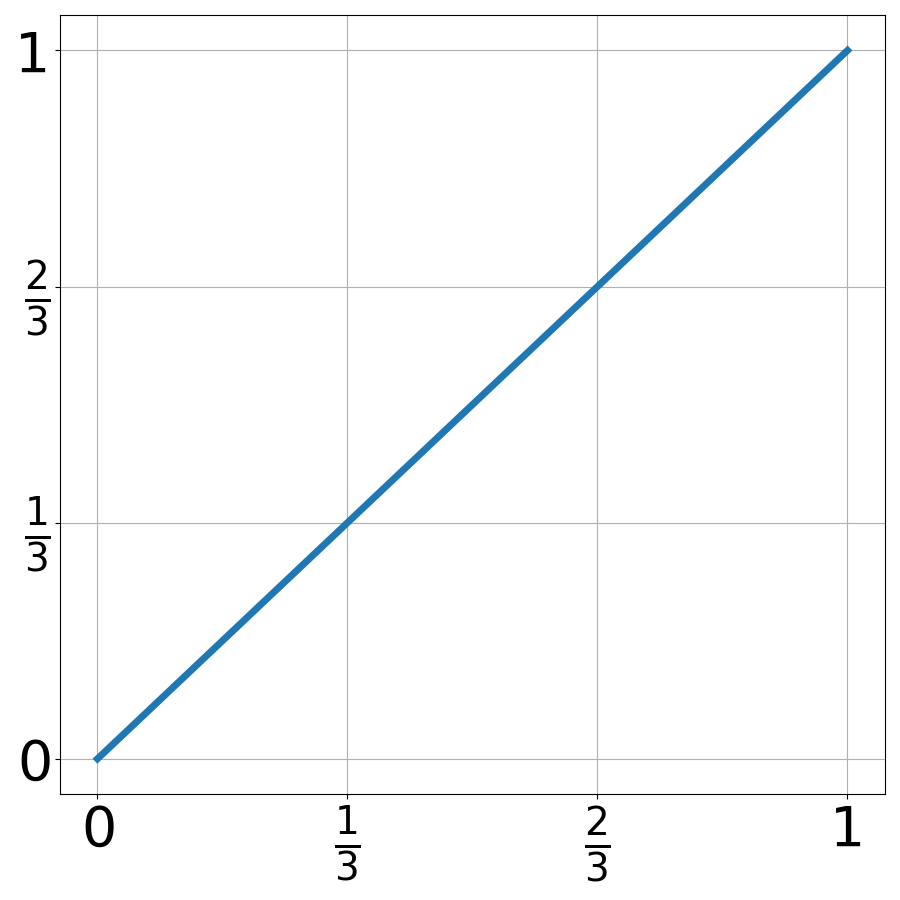
\includegraphics[width=\linewidth]{UA_Section_6_2_Figure_1.png}
                \caption{\( f_0 \) on \( [0, 1] \)}
                \label{fig:1sub1}
            \end{subfigure}%
            \begin{subfigure}{0.47\textwidth}
                \centering
                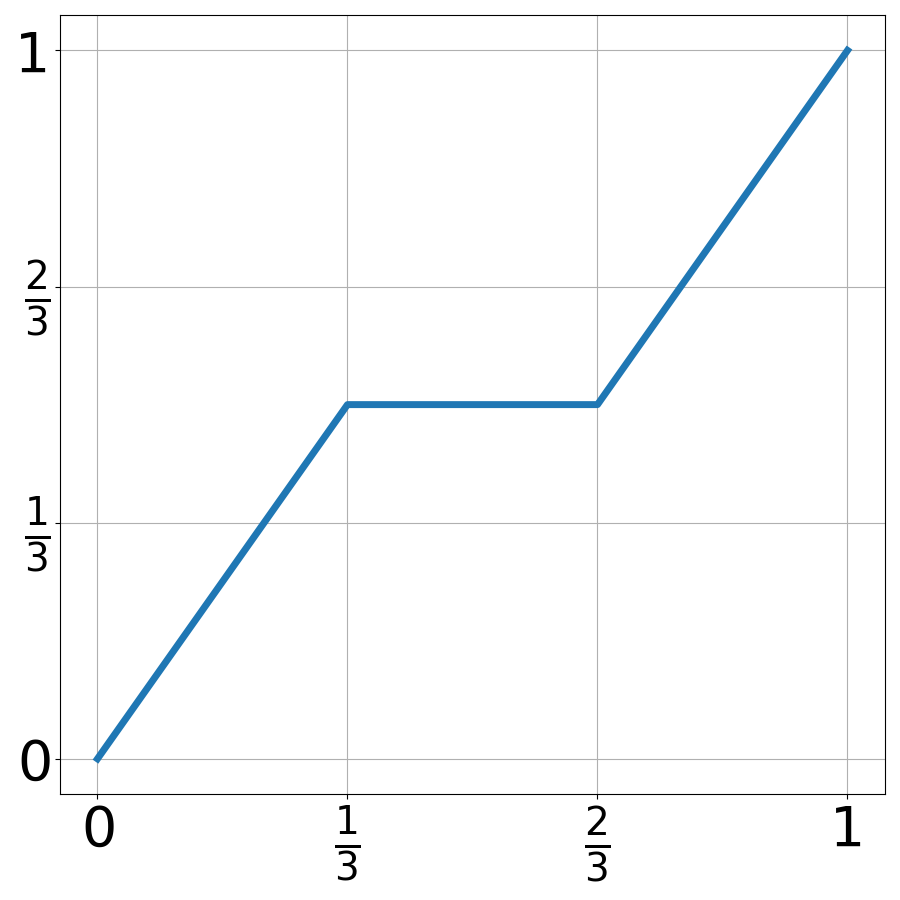
\includegraphics[width=\linewidth]{UA_Section_6_2_Figure_2.png}
                \caption{\( f_1 \) on \( [0, 1] \)}
                \label{fig:1sub2}
            \end{subfigure}

            \begin{subfigure}{0.47\textwidth}
                \centering
                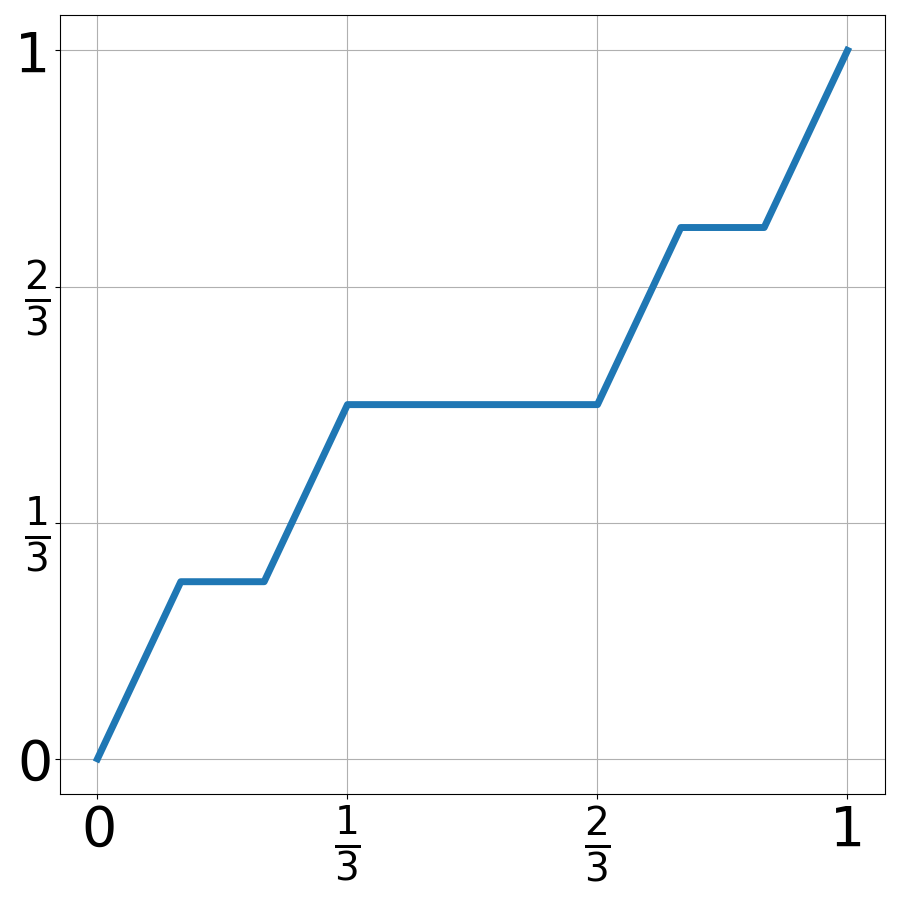
\includegraphics[width=\linewidth]{UA_Section_6_2_Figure_3.png}
                \caption{\( f_2 \) on \( [0, 1] \)}
                \label{fig:1sub3}
            \end{subfigure}%
            \begin{subfigure}{0.47\textwidth}
                \centering
                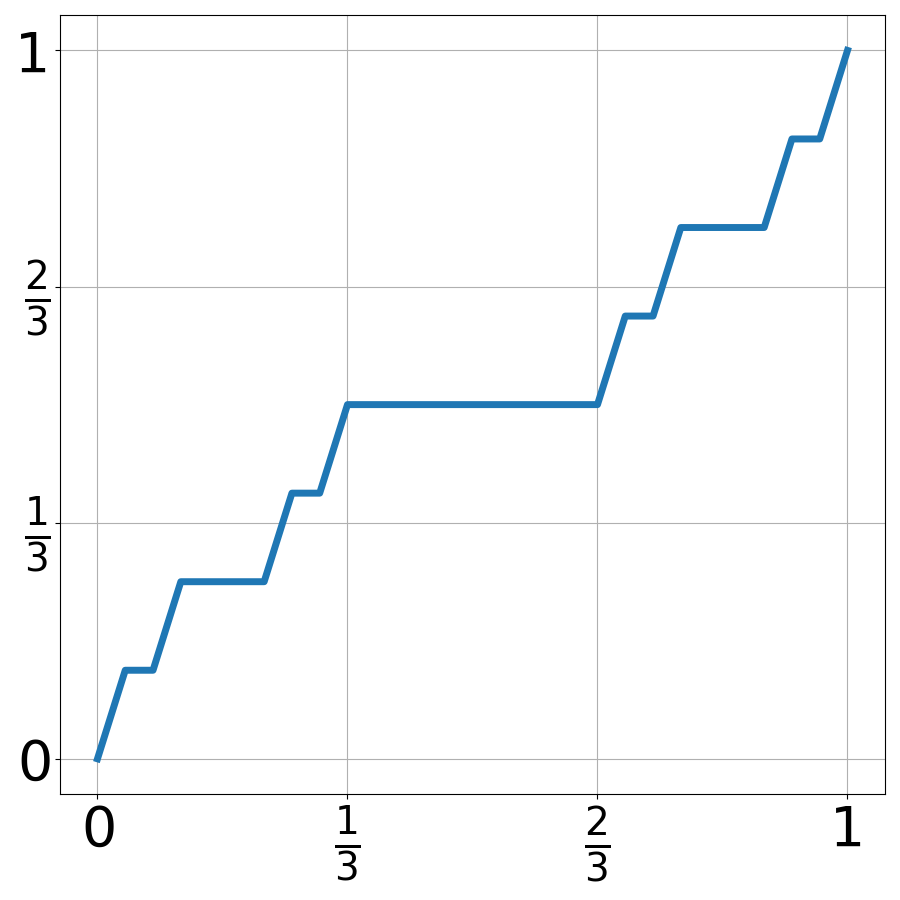
\includegraphics[width=\linewidth]{UA_Section_6_2_Figure_4.png}
                \caption{\( f_3 \) on \( [0, 1] \)}
                \label{fig:1sub4}
            \end{subfigure}
            
            \caption{\( f_0, f_1, f_2 \), and \( f_3 \) on \( [0, 1] \)}
            \label{fig:1}
        \end{figure}

        \item The sequence \( (f_n) \) is defined by
        \[
            f_n(x) = \begin{cases}
                \tfrac{1}{2} f_{n-1}(3x) & \text{if } 0 \leq x \leq \tfrac{1}{3}, \\
                f_{n-1}(x) & \text{if } \tfrac{1}{3} < x < \tfrac{2}{3}, \\
                \tfrac{1}{2} f_{n-1}(3x - 2) + \tfrac{1}{2} & \text{if } \tfrac{2}{3} \leq x \leq 1
            \end{cases}
        \]
        for \( n \geq 2 \).
        
        Let us first show by induction that \( \abs{f_{n+1}(x) - f_n(x)} \leq \tfrac{1}{6} \cdot \tfrac{1}{2^n} \) for all \( n \in \N \). For the base case \( n = 1 \), by studying the graphs of \( f_1 \) and \( f_2 \) in \Cref{fig:2} we can see that the maximum of \( \abs{f_2(x) - f_1(x)} \) is \( \tfrac{1}{12} \), which is achieved at \( x = \tfrac{1}{9}, \tfrac{2}{9}, \tfrac{7}{9}, \tfrac{8}{9} \).
        \begin{figure}[H]
            \centering
            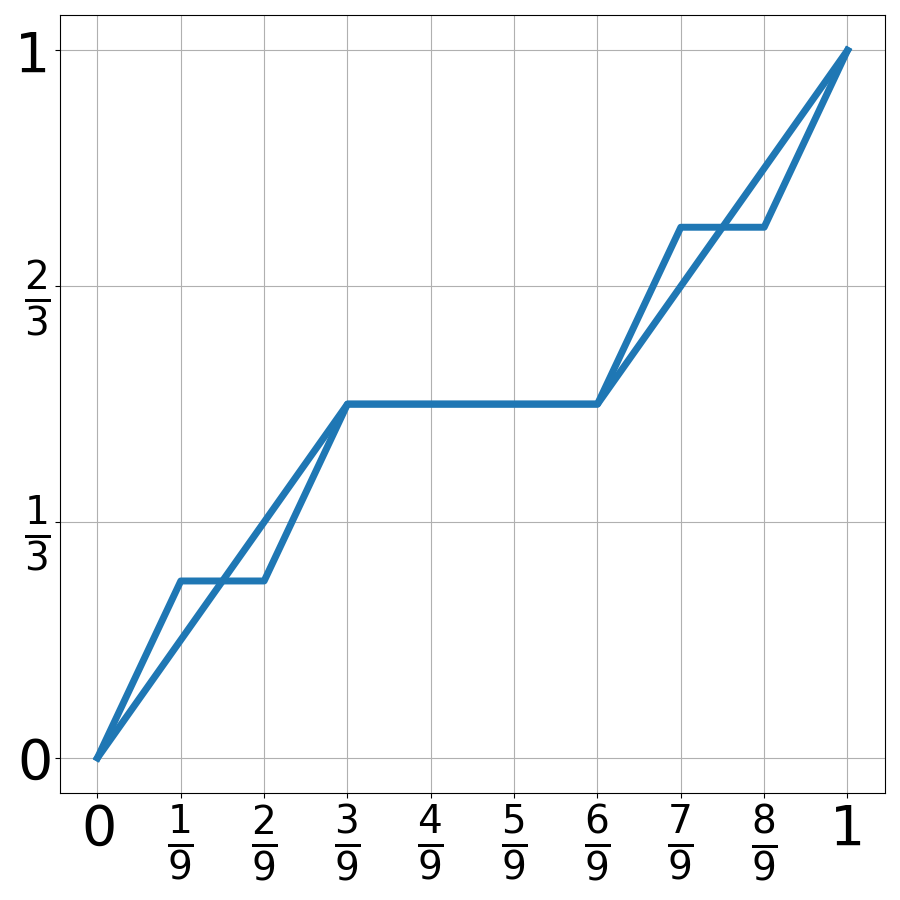
\includegraphics[width=0.5\linewidth]{UA_Section_6_2_Figure_5.png}
            \caption{\( f_0 \) and \( f_1 \) on \( [0, 1] \)}
            \label{fig:2}
        \end{figure}
        Suppose that \( \abs{f_{n+1}(x) - f_n(x)} \leq \tfrac{1}{6} \cdot \tfrac{1}{2^n} \) for some \( n \in \N \). There are three cases to consider.
        \begin{description}
            \item[Case 1.] For \( 0 \leq x \leq \tfrac{1}{3} \), we have \( f_{n+2}(x) = \tfrac{1}{2} f_{n+1}(3x) \) and \( f_{n+1}(x) = \tfrac{1}{2} f_n(3x) \). It follows that
            \[
                \abs{f_{n+2}(x) - f_{n+1}(x)} = \abs{\tfrac{1}{2} f_{n+1}(3x) - \tfrac{1}{2} f_n(3x)} = \tfrac{1}{2} \abs{f_{n+1}(3x) - f_n(3x)} \leq \tfrac{1}{6} \cdot \tfrac{1}{2^{n+1}},
            \]
            where we have used the induction hypothesis for the last inequality.

            \item[Case 2.] For \( \tfrac{1}{3} \leq x \leq \tfrac{2}{3} \), we have \( f_{n+2}(x) = f_{n+1}(x) \) and thus \( \abs{f_{n+2}(x) - f_{n+1}(x)} = 0 \).

            \item[Case 3.] For \( \tfrac{2}{3} \leq x \leq 1 \), we have \( f_{n+2}(x) = \tfrac{1}{2} f_{n+1}(3x - 2) + \tfrac{1}{2} \) and \( f_{n+1}(x) = \tfrac{1}{2} f_n(3x - 2) + \tfrac{1}{2} \). It follows that
            \begin{multline*}
                \abs{f_{n+2}(x) - f_{n+1}(x)} = \abs{\tfrac{1}{2} f_{n+1}(3x - 2) - \tfrac{1}{2} f_n(3x - 2)} \\[2mm]
                = \tfrac{1}{2} \abs{f_{n+1}(3x - 2) - f_n(3x - 2)} \leq \tfrac{1}{6} \cdot \tfrac{1}{2^{n+1}},
            \end{multline*}
            where we have used the induction hypothesis for the last inequality.
        \end{description}
        This completes the induction step and thus \( \abs{f_{n+1}(x) - f_n(x)} \leq \tfrac{1}{6} \cdot \tfrac{1}{2^n} \) for all \( n \in \N \).

        The inequality just proven implies that for any \( x \in [0, 1] \) and positive integers \( n > m \), we have
        \[
            \abs{f_n(x) - f_m(x)} \leq \sum_{j=m}^{n-1} \abs{f_{j+1}(x) - f_j(x)} \leq \frac{1}{6} \sum_{j=m}^{n-1} \frac{1}{2^j}. \tag{1}
        \]
        Let \( \epsilon > 0 \) be given. Since the series \( \sum_{j=0}^{\infty} \tfrac{1}{2^j} \) is convergent, its sequence of partial sums is a Cauchy sequence. Consequently, there exists an \( N \in \N \) such that \( \sum_{j=m}^{n-1} \tfrac{1}{2^j} < \epsilon \) for all \( n > m \geq N \). It follows from (1) that \( \abs{f_n(x) - f_m(x)} < \epsilon \) for all \( x \in [0, 1] \) and \( n > m \geq N \). Theorem 6.2.5 allows us to conclude that \( (f_n) \) converges uniformly on \( [0, 1] \).

        \item It is clear from the graphs in \Cref{fig:1} that each \( f_n \) is a continuous increasing function satisfying \( f(0) = 0 \) and \( f(1) = 1 \); it is straightforward to argue this by induction. It follows from the Continuous Limit Theorem (Theorem 6.2.6), Lemma 2 from the solution to \Cref{ex:10}, and the uniform convergence \( f_n \to f \) that \( f \) is a continuous increasing function satisfying \( f(0) = 0 \) and \( f(1) = 1 \).

        Let \( x \in [0, 1] \setminus C \) be given. By De Morgan's Laws, we have
        \[
            [0, 1] \setminus C = [0, 1] \setminus \paren{ \bigcap_{m=1}^{\infty} C_m } = \bigcup_{m=1}^{\infty} \paren{ [0, 1] \setminus C_m }.
        \]
        Thus \( x \in [0, 1] \setminus C_m \) for some \( m \in \N \). We constructed the sequence \( (f_n) \) in such a way that \( f_n \) is constant on the open set \( [0, 1] \setminus C_m \) for all \( n \geq m \); the uniform convergence \( f_n \to f \) then implies that \( f \) is constant on \( [0, 1] \setminus C_m \) for any \( m \in \N \). The openness of \( [0, 1] \setminus C_m \) implies that there is some open interval \( I \) contained in \( [0, 1] \setminus C_m \) and containing \( x \) such that \( f \) is constant on \( I \). It follows that \( f \) is differentiable at \( x \) and moreover that \( f'(x) = 0 \).
    \end{enumerate}
\end{solution}

\begin{exercise}
\label{ex:13}
    Recall that the Bolzano-Weierstrass Theorem (Theorem 2.5.5) states that every bounded sequence of real numbers has a convergent subsequence. An analogous statement for bounded sequences of functions is not true in general, but under stronger hypotheses several different conclusions are possible. One avenue is to assume the common domain for all of the functions in the sequence is countable. (Another is explored in the next two exercises.)

    Let \( A = \{ x_1, x_2, x_3, \ldots \} \) be a countable set. For each \( n \in \N \), let \( f_n \) be defined on \( A \) and assume there exists an \( M > 0 \) such that \( \abs{f_n(x)} \leq M \) for all \( n \in \N \) and \( x \in A \). Follow these steps to show that there exists a subsequence of \( (f_n) \) that converges pointwise on \( A \).
    \begin{enumerate}
        \item Why does the sequence of real numbers \( f_n(x_1) \) necessarily contain a convergent subsequence \( (f_{n_k}) \)? To indicate that the subsequence of functions \( (f_{n_k}) \) is generated by considering the values of the functions at \( x_1 \), we will use the notation \( f_{n_k} = f_{1,k} \).

        \item Now, explain why the sequence \( f_{1,k}(x_2) \) contains a convergent subsequence.

        \item Carefully construct a nested family of subsequences \( (f_{m,k}) \), and show how this can be used to produce a single subsequence of \( (f_n) \) that converges at every point of \( A \).
    \end{enumerate}
\end{exercise}

\begin{solution}
    For the purposes of this exercise, let us adopt some more precise, if cumbersome, notation for sequences. A sequence in a non-empty set \( E \) is a function \( a : \N \to E \). A sequence \( b : \N \to E \) is a subsequence of \( a \) if there exists a strictly increasing function \( \theta : \N \to \N \) such that \( b = a \circ \theta \), i.e.\ such that \( b(n) = a(\theta(n)) \) for all \( n \in \N \). We shall write \( b \triangleleft a \) to mean that \( b \) is a subsequence of \( a \). Given this definition, it is clear that if \( c \) is a subsequence of \( b \) and if \( b \) is a subsequence of \( a \), then \( c \) is a subsequence of \( a \). In other words, \( \triangleleft \) is transitive.
    \begin{enumerate}
        \item Define \( a_0 : \N \to \R^A \) (where \( \R^A \) is the collection of all functions from \( A \) to \( \R \)) by \( a_0(n) = f_n \). By assumption, the sequence of real numbers whose \( n \)\ts{th} term is \( [a_0(n)](x_1) \) is bounded. According to the Bolzano-Weierstrass Theorem, there then exists a strictly increasing function \( \theta_1 : \N \to \N \) such that \( \lim_{n \to \infty} [a_0(\theta_1(n))](x_1) = y_1 \) for some \( y_1 \in \R \). Define \( a_1 : \N \to \R^A \) by \( a_1 = a_0 \circ \theta_1 \). Note that \( a_1 \triangleleft a_0 \) and that
        \[
            \lim_{n \to \infty} [a_1(n)](x_1) = y_1.
        \]

        \item The sequence of real numbers whose \( n \)\ts{th} term is \( [a_1(n)](x_2) \) is bounded by assumption. According to the Bolzano-Weierstrass Theorem, there exists a strictly increasing function \( \theta_2 : \N \to \N \) such that \( \lim_{n \to \infty} [a_1(\theta_2(n))](x_2) = y_2 \) for some \( y_2 \in \R \). Define \( a_2 : \N \to \R^A \) by \( a_2 = a_1 \circ \theta_2 = a_0 \circ \theta_1 \circ \theta_2 \) and note that \( a_2 \triangleleft a_1 \triangleleft a_0 \). Note further that
        \[
            \lim_{n \to \infty} [a_2(n)](x_2) = y_2 \quand \lim_{n \to \infty} [a_2(n)](x_1) = y_1,
        \]
        since subsequences of convergent sequences converge to the same limit as the parent sequence.

        \item We continue in this manner, obtaining for each \( m \in \N \) a sequence \( a_m : \N \to \R^A \), a strictly increasing function \( \theta_m : \N \to \N \) such that \( a_m = a_{m-1} \circ \theta_m = a_0 \circ \theta_1 \circ \cdots \circ \theta_m \), and a real number \( y_m \) such that
        \[
            \lim_{n \to \infty} [a_m(n)](x_m) = y_m.    
        \]
        It follows that \( a_m \triangleleft a_{m-1} \triangleleft \cdots \triangleleft a_1 \triangleleft a_0 \), which implies that
        \[
            \lim_{n \to \infty} [a_m(n)](x_j) = y_j
        \]
        for each \( 1 \leq j \leq m \), since subsequences of convergent sequences converge to the same limit as the parent sequence.
        
        Define \( \Theta : \N \to \N \) by \( \Theta(n) = (\theta_1 \circ \cdots \circ \theta_n)(n) \); we claim that \( \Theta \) is strictly increasing. Indeed, let \( m < n \) be positive integers. Then
        \[
            m < n \leq \theta_n(n) \leq \cdots \leq (\theta_{m+1} \circ \cdots \circ \theta_n)(n),
        \]
        where we have used that \( n \leq \theta(n) \) for any strictly increasing function \( \theta : \N \to \N \). Now, a composition of strictly increasing functions is again a strictly increasing function. It follows that \( \theta_1 \circ \cdots \circ \theta_m \) is a strictly increasing function and hence that
        \[
            (\theta_1 \circ \cdots \circ \theta_m)(m) < (\theta_1 \circ \cdots \circ \theta_m \circ \cdots \circ \theta_n)(n),
        \]
        i.e.\ \( \Theta(m) < \Theta(n) \), as claimed.

        Define \( b : \N \to \R^A \) by \( b = a_0 \circ \Theta \), so that
        \[
            b(n) = (a_0 \circ \Theta)(n) = (a_0 \circ \theta_1 \circ \cdots \circ \theta_n)(n) = a_n(n).
        \]
        This is a subsequence of \( a_0 \) since \( \Theta \) is a strictly increasing function. This subsequence is sometimes known as the ``diagonal subsequence''; the following visualization can explain why.
        \[
            \begin{array}{c|cccc}
                a_1 & \textcolor{red}{a_1(1)} & a_1(2) & a_1(3) & \cdots \\
                a_2 & a_2(1) & \textcolor{red}{a_2(2)} & a_2(3) & \cdots \\
                a_3 & a_3(1) & a_3(2) & \textcolor{red}{a_3(3)} & \cdots \\
                \vdots & \vdots & \vdots & \vdots & \ddots
            \end{array}
        \]
        The \( m \)\ts{th} row corresponds to the sequence \( a_m \); note that each row is a subsequence of each row preceding it. The sequence \( b \) is obtained by taking the diagonal elements of this infinite array, highlighted in red.
        
        Our goal now is to show that \( b = (f_{\Theta(n)})_{n=1}^{\infty} \) converges pointwise on \( A \) to the function \( f : A \to \R \) given by \( f(x_m) = y_m \). Let \( m \in \N \) be given and note that for \( n \geq m + 1 \) we have
        \[
            b(n) = (a_0 \circ \Theta)(n) = (a_0 \circ \theta_1 \circ \cdots \circ \theta_n)(n) = (a_m \circ \theta_{m+1} \circ \cdots \circ \theta_n)(n) = (a_m \circ \Theta_m)(n),
        \]
        where \( \Theta_m : \{ m + 1, m + 2, \ldots \} \to \N \) is defined by
        \[
            \Theta_m(n) = (\theta_{m+1} \circ \cdots \circ \theta_n)(n).
        \]
        Similarly to how we showed that \( \Theta \) is strictly increasing, we can show that \( \Theta_m \) is strictly increasing. It follows that \( b \) is eventually a subsequence of \( a_m \) and hence that
        \[
            \lim_{n \to \infty} [b(n)](x_m) = \lim_{n \to \infty} [a_m(n)](x_m) = y_m.
        \]
    \end{enumerate}
\end{solution}

\begin{exercise}
\label{ex:14}
    A sequence of functions \( (f_n) \) defined on a set \( E \subseteq \R \) is called \textit{equicontinuous} if for every \( \epsilon > 0 \) there exists a \( \delta > 0 \) such that \( \abs{f_n(x) - f_n(y)} < \epsilon \) for all \( n \in \N \) and \( \abs{x - y} < \delta \) in \( E \).
    \begin{enumerate}
        \item What is the difference between saying that a sequence of functions \( (f_n) \) is equicontinuous and just asserting that each \( f_n \) in the sequence is individually uniformly continuous?

        \item Give a qualitative explanation for why the sequence \( g_n(x) = x^n \) is not equicontinuous on \( [0, 1] \). Is each \( g_n \) uniformly continuous on \( [0, 1] \)?
    \end{enumerate}
\end{exercise}

\begin{solution}
    \begin{enumerate}
        \item If \( (f_n) \) is equicontinuous, then for a given \( \epsilon > 0 \) the \( \delta > 0 \) that we obtain depends only on \( \epsilon \); if instead we only have that each \( f_n \) is individually uniformly continuous, then the \( \delta \) may very well depend on \( n \). In symbols, \( (f_n) \) is equicontinuous if
        \[
            (\forall \epsilon > 0) (\exists \delta > 0) (\forall n \in \N) \big( (x, y \in E \text{ and } \abs{x - y} < \delta) \implies \abs{f_n(x) - f_n(y)} < \epsilon \big),
        \]
        whereas each \( f_n \) is individually uniformly continuous if
        \[
            (\forall n \in \N) (\forall \epsilon > 0) (\exists \delta > 0) \big( (x, y \in E \text{ and } \abs{x - y} < \delta) \implies \abs{f_n(x) - f_n(y)} < \epsilon \big).
        \]
        Notice the order of the quantifiers.

        \item The issue occurs near 1; no matter how small \( \delta \) is taken, it is possible to take \( n \) large enough and \( x \) within \( \delta \) of 1 such that \( f_n(x) \) and \( f_n(1) \) are far apart. Geometrically, the slope of \( f_n \) gets very steep near 1 as we increase \( n \). To be more precise, let \( \delta > 0 \) be given, take \( n \in \N \) such that \( \tfrac{1}{n} < \delta \), and set \( x = 1 - \tfrac{1}{n} \). Then \( 1 - x < \delta \) and
        \[
            \abs{f_n(1) - f_n(x)} = 1 - \paren{ 1 - \frac{1}{n} }^n \geq 1 - e^{-1} > 0.
        \]
        We are using here that \( \paren{ 1 - \tfrac{1}{n} }^n \) is an increasing sequence which converges to \( e^{-1} \).

        Each \( g_n \) is uniformly continuous on \( [0, 1] \) by Theorem 4.4.7.
    \end{enumerate}
\end{solution}

\begin{exercise}[Arzela-Ascoli Theorem]
\label{ex:15}
    For each \( n \in \N \), let \( f_n \) be a function defined on \( [0, 1] \). If \( (f_n) \) is bounded on \( [0, 1] \)---that is, there exists an \( M > 0 \) such that \( \abs{f_n(x)} \leq M \) for all \( n \in \N \) and \( x \in [0, 1] \)---and if the collection of functions \( (f_n) \) is equicontinuous (\Cref{ex:14}), follow these steps to show that \( (f_n) \) contains a uniformly convergent subsequence.
    \begin{enumerate}
        \item Use \Cref{ex:13} to produce a subsequence \( (f_{n_k}) \) that converges at every rational point in \( [0, 1] \). To simplify the notation, set \( g_k = f_{n_k} \). It remains to show that \( (g_k) \) converges uniformly on all of \( [0, 1] \).

        \item Let \( \epsilon > 0 \). By equicontinuity, there exists a \( \delta > 0 \) such that
        \[
            \abs{g_k(x) - g_k(y)} < \frac{\epsilon}{3}
        \]
        for all \( \abs{x - y} < \delta \) and \( k \in \N \). Using this \( \delta \), let \( r_1, r_2, \ldots, r_m \) be a \textit{finite} collection of rational points with the property that the union of the neighborhoods \( V_{\delta}(r_i) \) contains \( [0, 1] \).

        Explain why there must exist an \( N \in \N \) such that
        \[
            \abs{g_s(r_i) - g_t(r_i)} < \frac{\epsilon}{3}
        \]
        for all \( s, t \geq N \) and \( r_i \) in the finite subset of \( [0, 1] \) just described. Why does having the set \( \{ r_1, r_2, \ldots, r_m \} \) be finite matter?

        \item Finish the argument by showing that, for an arbitrary \( x \in [0, 1] \),
        \[
           \abs{g_s(x) - g_t(x)} < \epsilon   
        \]
        for all \( s, t \geq N \).
    \end{enumerate}
\end{exercise}

\begin{solution}
    \begin{enumerate}
        \item Since \( \Q \cap [0, 1] \) is countable, \Cref{ex:13} implies the existence of the desired subsequence \( (g_k) \).

        \item Consider the open cover \( [0, 1] \subseteq \bigcup_{r \in \Q \cap [0, 1]} V_{\delta}(r) \). Since \( [0, 1] \) is compact, there exist points \( r_1, r_2, \ldots, r_m \) in \( \Q \cap [0, 1] \) such that \( V_{\delta}(r_1) \cup \cdots \cup V_{\delta}(r_m) \) contains \( [0, 1] \).

        Let \( 1 \leq i \leq m \) be given. Since \( (g_k) \) converges at every rational point in \( [0, 1] \), the sequence \( (g_k(r_i)) \) must be a Cauchy sequence. It follows that there exists an \( N_i \in \N \) such that
        \[
            s, t \geq N_i \implies \abs{g_s(r_i) - g_t(r_i)} < \frac{\epsilon}{3}.
        \]
        Thus the desired \( N \in \N \) is \( N = \max \{ N_1, \ldots, N_m \} \); the finiteness of \( \{ r_1, \ldots, r_m \} \) ensures this maximum exists.

        \item Let \( x \in [0, 1] \) be given, so that \( x \in V_{\delta}(r_i) \) for some \( 1 \leq i \leq m \), and let \( s, t \geq N \) be given. Then
        \[
            \abs{g_s(x) - g_t(x)} \leq \abs{g_s(x) - g_s(r_i)} + \abs{g_t(x) - g_t(r_i)} + \abs{g_s(r_i) - g_t(r_i)} = \tfrac{\epsilon}{3} + \tfrac{\epsilon}{3} + \tfrac{\epsilon}{3} = \epsilon,
        \]
        where we have used that \( \abs{x - r_i} < \delta \).
    \end{enumerate}
\end{solution}

\noindent \hrulefill

\noindent \hypertarget{ua}{\textcolor{blue}{[UA]} Abbott, S. (2015) \textit{Understanding Analysis.} 2\ts{nd} edition.}

\end{document}